\section{Лекция 13.}

\subsection{Два вида норм индукции}

\deff{def:} Принцип математической индукции

Какое бы ни было $\varphi(x)$, если $\varphi(0)$ и при всех $x$ выполнено $\varphi(x)\rightarrow \varphi(x')$, то
при всех $x$ выполнено и само $\varphi(x)$.

\deff{def:} Принцип полной математической индукции

Какое бы ни было $\psi(x)$, если $\psi(0)$ и при всех $x$ выполнено $(\forall t.t \leq x \rightarrow \psi(t))\rightarrow \psi(x')$, то
при всех $x$ выполнено и само $\psi(x)$.


\thmm{Теорема.} Принципы математической индукции эквивалентны

\textbf{Доказательство:}

$(\Rightarrow)$ взяв $\varphi := \psi$, имеем выполненность $\varphi(x)\rightarrow\varphi(x')$, значит, $\forall x.\psi(x)$. 

$(\Leftarrow)$ возьмём $\psi(x) := \forall t.t\le x\rightarrow\varphi(t)$.

\subsection{Наследственные подмножества}

\deff{def:} Назовём \textbf{вполне упорядоченное отношением} $(\in)$ множество $S$ наследственным подмножеством $A$, если 
$\forall x.x \in A \rightarrow (\forall t.t \in x \rightarrow t \in S) \rightarrow x \in S$.


\thmm{Теорема.} Единственным наследственным подмножеством вполне упорядоченного множества является оно само.

\textbf{Доказательство:}

Пусть $B \subseteq A$ --- наследственное и $B \ne A$.
Тогда существует $a = \min (A \setminus B)$. Тогда $(\forall t.t \in a \rightarrow t \in B) \rightarrow a \in B$ по наследственности $B$,
и выполнено $\forall t.t \in a \rightarrow t \in B$ (по минимальности $a$). Значит, $a \in B$.

\hfill Q.E.D.

\subsection{Трансфинитная индукция}

\thmm{Теорема.Ограниченная трансфинитная индукция} Если для $\varphi(x)$ (некоторого утверждения
теории множеств) и некоторого ординала $\varepsilon$ (ограничения) выполнено
$\forall x.x \in \varepsilon \rightarrow (\forall t.t \in x \rightarrow \varphi(t)) \rightarrow \varphi(x)$,
то $\forall x.x \in \varepsilon \rightarrow \varphi(x)$.


\textbf{Доказательство:}

Рассмотрим $S = \{ x\in \varepsilon\ |\ \varphi(x) \}$. Тогда $x \in S$ равносильно 
$x\in\varepsilon\with\varphi(x)$.
Тогда перепишем: $\forall e.e \in \varepsilon \rightarrow (\forall x.x \in e \rightarrow x \in S) \rightarrow e \in S$.
Отсюда по теореме о наследственных множествах $S = \varepsilon$.


\hfill Q.E.D.

\thmm{Теорема. Неограниченная трансфинитная индукция}

Если для $\varphi(x)$ (некоторого утверждения
теории множеств) выполнено
$\forall x.\text{ординал}(x) \rightarrow (\forall t.t \in x \rightarrow \varphi(t)) \rightarrow \varphi(x)$,
то $\forall x.\text{ординал}(x) \rightarrow \varphi(x)$.


\thmm{Теорема. Альтернативная формулировка.} 

Для ординала $\varepsilon$ подмножество $S \in \varepsilon$ --- наследственное, если и только если одновременно:\\
Если $x \in \varepsilon$ и $x = \varnothing$, то $x \in S$;\\
Если $x \in \varepsilon$ и существует $y$: $y' = x$, то $y \in S \rightarrow x \in S$;\\
Если $x \in \varepsilon$ и $x$ --- предельный, то $(\forall t.t \in x \rightarrow t \in S) \rightarrow (x \in S)$.

\textbf{Доказательство:}

$(\Rightarrow)$ очевидно. Докажем $(\Leftarrow)$: пусть $S$ не наследственное: 
$E := \{e \in \varepsilon \ |\  (\forall t.t \in e \rightarrow t \in S) \with e \notin S \}$
и $E \ne \varnothing$. Тогда пусть $e = \min E$.

\begin{enumerate}
\item $e = \varnothing$ или предельный. Тогда $(\forall t.t \in e \rightarrow t \in S) \rightarrow (e \in S)$.
\item $e = y'$. Тогда $y \in \varepsilon$ ($\varepsilon$ --- ординал) и 
$(\forall t.t \in y \rightarrow t \in S) \rightarrow (y \in S)$ (так как $e$ минимальный, для которого $S$ не наследственное).
По условию, $(y \in S) \rightarrow (e \in S)$, отсюда $(\forall t.t \in e \rightarrow t \in S) \rightarrow (e \in S)$.

\begin{center}
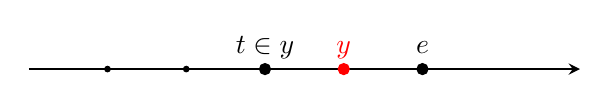
\begin{tikzpicture}
\draw[thick,-stealth] (0,0) -- (7,0); 
\filldraw (2,0) circle (1pt);
\filldraw (1,0) circle (1pt);
\filldraw (3,0) node[above] {$t \in y$} circle (2pt);
\filldraw[red] (4,0) node[above] {$y$} circle (2pt) ;
\filldraw (5,0) node[above] {$e\vphantom{y}$} circle (2pt) ;
\end{tikzpicture}
\end{center}

\end{enumerate}

\hfill Q.E.D.


Пример применения: $\alpha\cdot\alpha = \alpha$ при $\alpha \ge \aleph_0$

\thmm{Теорема.} Если $\alpha$ --- кардинальное число, $\alpha \ge \aleph_0$, 
то $\alpha\cdot\alpha = \alpha$.

\textbf{Доказательство:}

Трансфинитная индукция: $\varphi(x) := x < \omega \vee x \cdot x = x$
\begin{enumerate}
\item База: $x = \varnothing$. Тогда 
$\varphi(\varnothing) \equiv \varnothing < \omega \vee |\varnothing \times \varnothing| = \varnothing$,
что доказуемо.
\item Переход: $\forall y.y < x \rightarrow \varphi(y)$, тогда $\varphi(x)$. Три случая:
\begin{enumerate}
\item $x < \omega$. Тогда $\varphi(x)$ истинно (аналогично базе).
\item $x = \omega$. Счётный случай (рассмотрим отдельно).
\item $x > \omega$. Общий случай (рассмотрим отдельно).
\end{enumerate}
\end{enumerate}


Cчётный случай: $\omega < \omega \vee |\omega \cdot \omega| = \omega$

Тогда $\omega \times \omega$ упорядочим так: $\langle p,q \rangle \prec \langle s,t \rangle$,
если \begin{enumerate}
\item $\max(p,q) < \max(s,t)$
\item $\max(p,q) = \max(s,t)$ и $q < t$
\item $\max(p,q) = \max(s,t)$, $q = t$ и $p < s$
\end{enumerate}
Очевидно, можно построить биекцию между так упорядоченными значениями и $\omega$.

\begin{center}
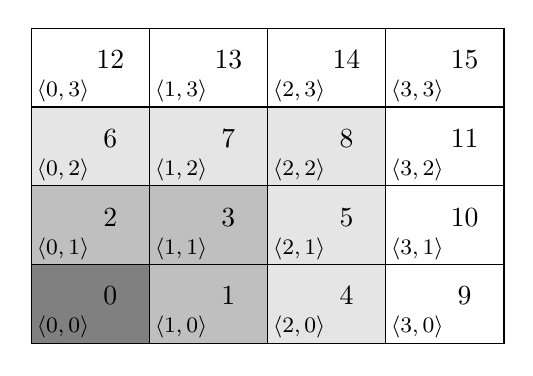
\begin{tikzpicture}
\filldraw[gray!20] (0,0) -- (4.5, 0) -- (4.5, 3) -- (0, 3) -- cycle;
\filldraw[gray!50] (0,0) -- (3, 0) -- (3, 2) -- (0, 2) -- cycle;
\filldraw[gray] (0,0) -- (1.5, 0) -- (1.5, 1) -- (0, 1) -- cycle;

\foreach \x in {0, 1, 2, 3} {
	\foreach \y in {0, 1, 2, 3} {
                \node at (1.5*\x + 1, \y + 0.6) {
			\pgfmathparse{(max(\x,\y))*(max(\x,\y)) + \y + ((\y+1)==(max(\x,\y)+1))*\x}%
			\pgfmathprintnumber{\pgfmathresult}%
		};
		\node at (1.5*\x + 0.4, \y + 0.2) {\footnotesize $\langle \x,\y \rangle$};
		\draw (1.5*\x, \y) -- (1.5*\x +1.5, \y) -- (1.5*\x +1.5, \y +1) -- (1.5*\x, \y +1) -- cycle;
	}
}
\end{tikzpicture}
\end{center}

Общий случай: $|\alpha \cdot \alpha| = \alpha$

Аналогично счётному случаю, $\alpha \times \alpha$ упорядочим так: $\langle p,q \rangle \prec \langle s,t \rangle$,
если \begin{enumerate}
\item $p \cup q < s \cup t$
\item $p \cup q = s \cup t$ и $q < t$
\item $p \cup q = s \cup t$, $q = t$ и $p < s$
\end{enumerate}

\begin{itemize}
\item Легко заметить, что это --- линейный порядок (показав, что $p \not\prec q$ и $q \not\prec p$ влечёт $p = q$)
\item ... и полный порядок. Найти наименьший в $S \ne \varnothing$ возможно, рассмотрев $m_1 := \min \{ p \cup q\ |\ \langle p,q \rangle \in S\}$ и
$M_1 := \{ \langle p,q\rangle\ |\ \langle p,q \rangle \in S, p \cup q = m_1\}$,
затем $m_2 := \min \{q\ |\ \langle p,q \rangle \in M_1 \}$,
$M_2 := \{\langle p,q\rangle\ |\ \langle p,q \rangle \in M_1, q = m_2\}$.
Тогда требуемым наименьшим в $S$ будет $\min \{ p\ |\ \langle p,q \rangle \in M_2\}$
\item Тогда $\langle \alpha\times\alpha, (\prec)\rangle$ соответствует какой-то ординал $\tau$ 
и сохраняющая порядок биекция $t: \tau\rightarrow\alpha\times\alpha$. 
\item Заметим, что $x < \omega$ тогда и только тогда, когда $\cup(\cup t(x)) < \omega$
(очевидно из того, что $|\{z\ |\ \text{ординал}(z), z < x\}|=|\{p\ |\ p \prec t(x)\}|$).
\item Покажем, что $|\tau| = \alpha$.
\end{itemize}

Докажем $\tau = \alpha$

Очевидно, что $\tau \ge \alpha$ (так как $|\tau| = |\alpha\times\alpha| \ge \alpha$). Но пусть $\tau > \alpha$.
\begin{itemize}
\item Тогда $t(\alpha) = \langle\zeta,\eta\rangle$ определено (у $\alpha$ есть образ).
\item Пусть $\sigma := \zeta \cup \eta$. Очевидно, $\langle \zeta, \eta \rangle \preceq \langle \sigma,\sigma \rangle$
и $\sigma \in \alpha$.
\item Каков образ $t$ на этом начальном отрезке?
$\{t(x)\ |\ x < \alpha\} \subseteq \{\langle p,q\rangle\ |\ p,q \le \sigma\}$.
Поэтому $\alpha \le |(\sigma+1)\times(\sigma+1)|$. 
\item С другой стороны, $\sigma < \alpha$. Поскольку $\alpha$ --- кардинал (т.е., в частности, предельный ординал), 
то $\sigma+1 < \alpha$ и $|\sigma+1| < \alpha$. 
\item По предположению индукции, $|\sigma+1|<\omega \vee |\sigma+1| = |\sigma+1|\cdot|\sigma+1|$,
по свойствам $(\prec)$ имеем $\sigma\ge\omega$.
\item Отсюда $\alpha \le |(\sigma+1)\times(\sigma+1)| = |\sigma+1| < \alpha$, что невозможно.
\end{itemize}

\hfill Q.E.D.

\subsection{Теорема о непротиворечивости формальной арифметики}

\deff{def:} Введем исчисление $S_\infty$

\begin{enumerate}
\item Язык: связки $\neg$, $\vee$, $\forall$, $=$; нелогические символы: $(+)$,$(\cdot)$,$(')$,$0$; переменные: $x$.
\item Аксиомы: все истинные формулы вида $\theta_1=\theta_2$; все истинные отрицания формул вида $\neg\theta_1=\theta_2$
($\theta_i$ --- термы без переменных).
\item Структурные (слабые) правила:
$$\infer{\zeta\vee\beta\vee\alpha\vee\delta}{\zeta\vee\alpha\vee\beta\vee\delta} \quad\quad
\infer{\alpha\vee\delta}{\alpha\vee\alpha\vee\delta}$$

Сильные правила
$$\infer{\alpha\vee\beta}{\beta}\quad
\infer{\neg(\alpha\vee\beta)\vee\delta}{\neg\alpha\vee\delta\quad\neg\beta\vee\delta}\quad
\infer{\neg\neg\alpha\vee\delta}{\alpha\vee\delta}\quad
\infer{(\neg\forall x.\alpha)\vee\delta}{\neg\alpha[x := \theta]\vee\delta}\quad$$

Формулы в правилах, обозначенные буквами $\zeta$ и $\delta$, называются боковыми и могут отсутствовать.



\item Бесконечная индукция:
$$\infer{(\forall x.\alpha)\vee\delta}{\alpha[x:=\overline{0}]\vee\delta
                                  \quad\alpha[x:=\overline{1}]\vee\delta
                                  \quad\alpha[x:=\overline{2}]\vee\delta\quad\dots}$$

\item Сечение:
$$\infer{\zeta\vee\delta}{\zeta\vee\alpha\quad\quad\neg\alpha\vee\delta}$$
Здесь $\alpha$ --- секущая формула, число связок в $\neg\alpha$ --- степень сечения.\\
В отличие от других правил, в правиле сечения хотя бы одна из боковых формул $\zeta$ или $\delta$ должна присутствовать.

\end{enumerate}

\begin{enumerate}
\item Доказательства образуют деревья.
\item Каждой формуле в дереве сопоставим порядковое число (ординал).
\item Порядковое число заключения любого неструктурного правила строго больше порядкового числа его посылок
(больше или равно в случае структурного правила).

$$\infer{(\neg\neg\forall x.\neg x'=0)_{\omega+1}}{\infer{(\forall x.\neg x' = 0)_\omega}{(\neg 1=0)_1\quad (\neg 2=0)_2 \quad (\neg 3=0)_4 \quad (\neg 4 = 0)_8 \dots}}$$

\item Существует конечная максимальная степень сечения в дереве (назовём её степенью вывода).
\end{enumerate}


\thmm{Теорема.} Если $\vdash_\text{фа}\alpha$, то $\vdash_\infty|\alpha|_\infty$ 

Обратное неверно: $$\infer{\forall x.\neg\omega_1(x,\overline{\ulcorner\sigma\urcorner})}
{\neg\omega_1(\overline{0},\overline{\ulcorner\sigma\urcorner})\quad\quad
 \neg\omega_1(\overline{1},\overline{\ulcorner\sigma\urcorner})\quad\quad
 \neg\omega_1(\overline{2},\overline{\ulcorner\sigma\urcorner})\quad\quad\dots}$$

\thmm{Теорема} Если Ф.А. противоречива, то противоречива и $S_\infty$

\subsection{Обратимость правил де Моргана, отрицания, бесконечной индукции}


$$\infer{\neg\alpha\vee\delta\quad\neg\beta\vee\delta\vphantom{overline{1}]}}{\neg(\alpha\vee\beta)\vee\delta}\quad
  \infer{\alpha\vee\delta\vphantom{overline{1}]}}{\neg\neg\alpha\vee\delta}\quad
  \infer{\alpha[x:=\overline{0}]\vee\delta
          \quad\alpha[x:=\overline{1}]\vee\delta
          \quad\alpha[x:=\overline{2}]\vee\delta\quad\dots}{(\forall x.\alpha)\vee\delta}
$$


\textbf{Доказательство:}

Например, формула вида $\neg\neg \alpha\vee\delta$.

Проследим историю $\neg\neg\alpha$; она могла быть получена:
\begin{enumerate}
\item ослаблением --- заменим $\neg\neg\alpha$ на $\alpha$ в этом узле и последующих.
\item отрицанием --- выбросим правило, заменим $\neg\neg\alpha$ на $\alpha$ в последующих.
\end{enumerate}

\begin{tabular}{ll}
\begin{minipage}{0.5\linewidth}
Изменённый вывод --- доказательство требуемого.
\end{minipage} &
\begin{minipage}{0.5\linewidth}
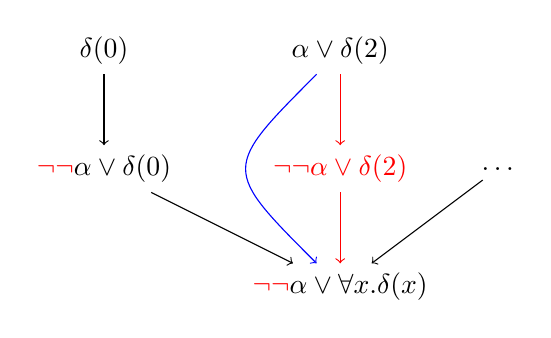
\begin{tikzpicture}
  \node at (-1.5,3) (J1) { $\delta(0)$ };
  \node at (1.5,3) (J2) { $\alpha\vee\delta(2)$ };
  \node at (-1.5,1.5) (I1) { ${\color{red}\neg\neg}\alpha\vee\delta(0)$ };
  \node at (1.5,1.5) (I2) { $\color{red}\neg\neg\alpha\vee\delta(2)$ };
  \node at (1.5,0) (C) { ${\color{red}\neg\neg}\alpha\vee\forall x.\delta(x)$ }; 
  \node at (3.5,1.5) (D) { $\dots$ };
  \draw[->] (J1) -- (I1); \draw[->] (I1) -- (C);
  \draw[red,->] (J2) -- (I2); \draw[red,->] (I2) -- (C);
  \draw[->] (D) -- (C);
  \draw[blue,->,bend right=20] (J2) .. controls (0,1.5) .. (C);
\end{tikzpicture}
\end{minipage}
\end{tabular}

\hfill Q.E.D.

\subsection{Устранение сечений}

\thmm{Теорема} Если $\alpha$ имеет вывод степени $m>0$ порядка $t$, то
можно найти вывод степени строго меньшей $m$ с порядком $2^t$.

\textbf{Доказательство:}

Трансфинитная индукция. Пусть для всех деревьев порядка $t_1 < t$ 
условие выполнено. Покажем, что оно выполнено для порядка $t$.
Рассмотрим заключительное правило. Это может быть...

\begin{enumerate}
\item Не сечение.
\item Сечение, секущая формула --- элементарная.
\item Сечение, секущая формула --- $\neg\alpha$.
\item Сечение, секущая формула --- $\alpha\vee\beta$.
\item Сечение, секущая формула --- $\forall x.\alpha$.
\end{enumerate}

\subsubsection{Случай 1. Не сечение}

$$\infer{(\alpha)_{t}}{(\pi_0)_{t_0}\quad(\pi_1)_{t_1}\quad(\pi_2)_{t_2}\quad\dots}$$
Заменим доказательства посылок $(\pi_i)_{t_i}$ на $(\pi'_i)_{2^{t_i}}$ по индукционному предположению.

\begin{enumerate}
\item Поскольку степени посылок $m'_i < m_i$, то $\max m'_i < \max m_i$.
\item Поскольку $t_i \le t$, то $2^{t_i} \le 2^t$.
\end{enumerate}

\subsubsection{Случай 5. Сечение с формулой вида $\forall x.\alpha$}

$$\infer{\zeta\vee\delta}{\zeta\vee\forall x.\alpha\quad\quad(\neg\forall x.\alpha)\vee\delta}$$
Причём степень и порядок выводов компонент, соответственно, $(m_1,t_1)$ и $(m_2,t_2)$.

\begin{enumerate}
\item По индукции, вывод $\zeta\vee\forall x.\alpha$ можно упростить до $(m_1',2^{t_1})$.
\item По обратимости, можно построить вывод $\zeta\vee\alpha[x := \theta]$ за $(m_1',2^{t_1})$.
\item В формуле $(\neg \forall x. \alpha)\vee\delta$ формула $\neg\forall x.\alpha$ получена
либо ослаблением, либо квантификацией из $\neg\alpha[x := \theta_k]\vee\delta_k$. 
\begin{enumerate}
\item Каждое правило квантификации заменим на:
$$\infer{\zeta\vee\delta_k}{\zeta\vee\alpha[x := \theta_k]\quad\quad(\neg\alpha[x := \theta_k])\vee\delta_k}$$
\item Остальные вхождения $\neg\forall x.\alpha$ заменим на $\zeta$ (в правилах ослабления).
\end{enumerate}
\item В получившемся дереве меньше степень --- так как в $\neg\alpha[x := \theta]$ меньше связок, чем в $\neg\forall x.\alpha$.
\end{enumerate}

\subsubsection{Случай 5. Как перестроим доказательство}

\begin{center}
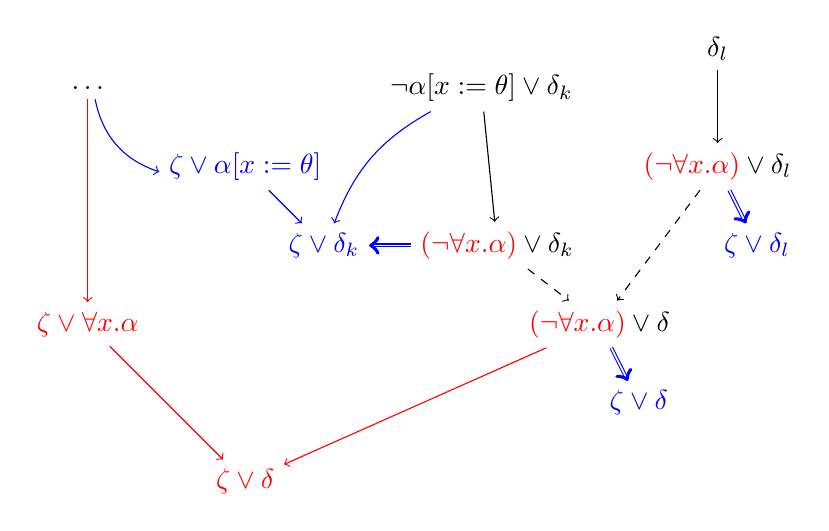
\begin{tikzpicture}
    \node (RRW) at (6,5.5) {$\delta_l$};
    \node (RR) at (6,4) {${\color{red}(\neg\forall x.\alpha)}\vee\delta_l$};
    \node (RRnew) at (6.5,3) {$\color{blue}\zeta\vee\delta_l$};
    \node (LL) at (-2,5) {$\dots$};

    \node (R) at (3.2,3) {${\color{red}(\neg\forall x.\alpha)}\vee\delta_k$};
    \node (Rnew) at (1,3) {$\color{blue}\zeta\vee\delta_k$};
    \node (RQ) at (3,5) {$\neg\alpha[x := \theta]\vee\delta_k$};
    \node (L1) at (0,4) {$\color{blue}\zeta\vee\alpha[x := \theta]$};
    \node (L) at (-2,2) {$\color{red}\zeta\vee\forall x.\alpha$};

    \node (CR) at (4.5,2) {${\color{red}(\neg\forall x.\alpha)}\vee\delta$};
    \node (CRnew) at (5,1) {$\color{blue}\zeta\vee\delta$};
    \node (C) at (0,0) {$\color{red}\zeta\vee\delta$};
    \draw[red,->] (L) -- (C);
    \draw[red,->] (LL) -- (L);
    \draw[red,->] (CR) -- (C);
    \draw[blue,->,bend right=30] (LL) to (L1);
    \draw[dashed,->] (R) -- (CR);
    \draw[dashed,->] (RR) -- (CR);
    \draw[double,->,blue] (RR) -- (RRnew);
    \draw[double,->,blue] (CR) -- (CRnew);
    \draw[double,->,blue] (R) -- (Rnew);
    \draw[->] (RRW) -- (RR);
    \draw[->] (RQ) -- (R);
    \draw[blue,->,bend right=20] (RQ) to (Rnew);
    \draw[blue,->] (L1) -- (Rnew);
\end{tikzpicture}
\end{center}

\subsection{Теорема об устранении сечений}

\deff{def:} Итерационная экспонента
$$(a\uparrow)^m(t
) = 
  \left\{
    \begin{array}{ll}     t,&m=0\\
                          a^{(a\uparrow)^{m-1}(t)},&m > 0
    \end{array}
  \right.
$$

\thmm{Теорема.} Если $\vdash_\infty\sigma$ степени $m$ порядка $t$, то найдётся доказательство без сечений
порядка $(2\uparrow)^m(t)$

\textbf{Доказательство:} В силу конечности $m$ воспользуемся индукцией по $m$ и теоремой об уменьшении степени.

\subsection{Порядок трансфинитной индукции}

\deff{def:} $\varepsilon_0$ --- неподвижная точка $\varepsilon_0 = \omega^{\varepsilon_0}$

Иначе говоря, $\varepsilon_0 = \{ \omega, \omega^\omega, \omega^{\omega^\omega}, (\omega \uparrow)^3(\omega), (\omega\uparrow)^4(\omega), \dots \}$.

Очевидно, что теорема об устранении сечений может быть доказана трансфинитной индукцией до ординала $\varepsilon_0$
(максимальный порядок дерева вывода, при правильной нумерации вершин).

\subsection{Непротиворечивость формальной арифметики}

\thmm{Лемма.} Если $\vdash_\infty\alpha$ и $\vdash_\infty\neg\alpha$, тогда $\vdash_\infty\neg 0=0$.

\thmm{Теорема.} $\not\vdash_\infty\neg 0=0$

\textbf{Доказательство:}


Пусть $\vdash_\infty\neg 0=0$, устраним сечения и рассмотрим заключительное правило.

\begin{enumerate}
\item Правило де Моргана? Нет отрицаний дизъюнкции ($\neg(\alpha\vee\beta)\vee\delta$).
\item Отрицание? Нет двойного отрицания ($\neg\neg\alpha\vee\delta$).
\item Бесконечная индукция или квантификация? Нет квантора.
\item Ослабление? Нет дизъюнкции ($\alpha \vee \beta$), хотя $\beta$ обязана присутствовать.
\item Сечение? Исключено по условию.
\end{enumerate}

То есть, неизбежно, $\neg 0=0$ --- аксиома, что также неверно.
